\chapter{Metodologia}
\label{chap:MatMet}

O Capítulo \ref{chap:ch1} apresentou alguns dos métodos encontrados na literatura para a representação computacional de formas a partir do seu contorno.  Em muitos casos, esses métodos apresentam parâmetros que requerem ajustes, sendo esse ajuste dependente da natureza da aplicação, ou seja,  das características da base de imagens e do propósito ao qual o sistema de reconhecimento se destina.

Os descritores entropia multiescala, apresentado no Capítulo \ref{chap:ch2}, e a energia de dobramento multiescala requerem o ajuste dos seguintes parâmetros: o número e os valores dos fatores de escala utilizados na representação das formas. Esse capítulo apresenta um método robusto e versátil para o ajuste desses parâmetros para customizar esses descritores em aplicações de classificação supervisionada e não supervisionada.   
 

\section{Ajuste de parâmetros}
A metodologia para escolha de parâmetros do descritor segue o esquema da Figura \ref{fig:Avaliacao}. Essa metodologia melhora a representação do descritor utilizando métodos de otimização evolutivos para minimizar uma função custo que corresponde a mediana do erro absoluto da silhouette dos descritores ($MAD$). O que motivou a escolha dessa função custo é sua robustez a valores extremos \cite{Rousseeuw:1987:2}, sendo sua equação 

\begin{equation}
\label{eq:mad}
MAD = \operatorname{mediana}\big(|s_i - 1|_{i =1,\:2,\:\cdots,\:L}\big)\text{,}
\end{equation}

\begin{figure*}[ht]
\centering
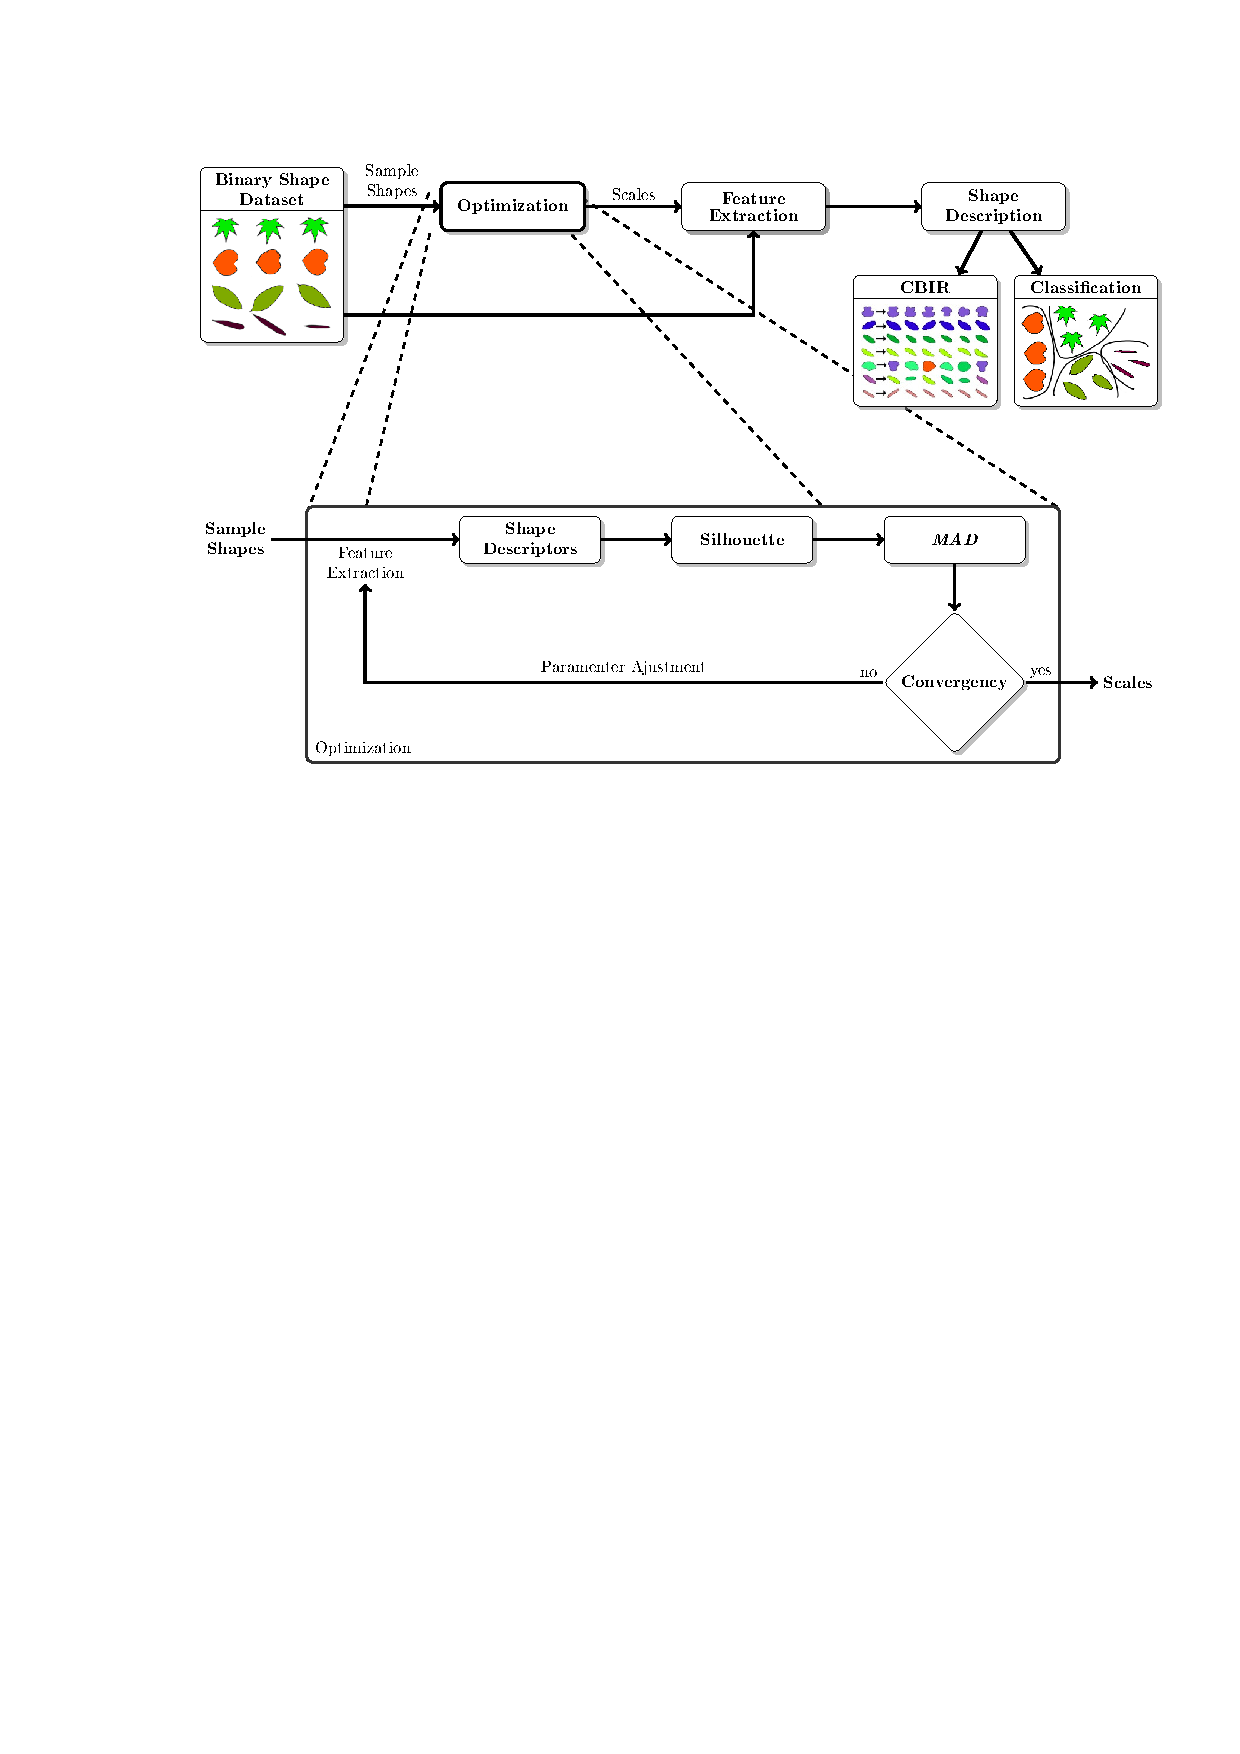
\includegraphics[width=\textwidth,trim = 14mm 164mm 0mm 24mm,clip]{Final_Flux.pdf}
\caption{The proposed approach for evolutionary optimization of a multiscale shape descriptor.} 
\label{fig:Avaliacao}
\end{figure*}

\noindent aonde $S = \{s_1,s_2,\cdots,s_L\}$ é o conjunto das \emph{silhouettes} calculadas para $L$ descritores de forma. Os operadores $|.|$  e {$mediana ( )$} retornam o valor absoluto e a mediana de um conjunto de valores, respectivamente.

A Silhouette \cite{Rousseeuw:1987} é uma medida de qualidade de agrupamentos que indica o grau de afinidade de uma amostra  a um agrupamento, levando em conta as distâncias médias entre-classes e intra-classes de um objeto $i$ atribuído a uma dada classe $A$. Logo, esta métrica é definida como 
\begin{equation}
s_i = \frac{b_i - a_i}{\max{(a_i,b_i)}} \in [-1,1],
\end{equation}

\noindent sendo $a_i$ a dissimilaridade média entre o objeto $i$ e os demais objetos pertencentes a mesma classe de $a_i$ e $b_i$ é a dissimilaridade média do objeto $i$ e a classe vizinha mais próxima de $i$, excluída sua própria classe. 

Essa métrica pode assumir valores no intervalo $[-1,1]$, sendo que valores negativos indicam que o grau de pertencimento de um objeto à classe que este fora atribuído é baixo. Já valores positivos indicam que o grau de pertencimento de um objeto à classe que este fora atribuído é alto. Um valor de silhouette próximo de zero indica que o objeto está na fronteira entre duas classes e que há, portanto, um grau de incerteza a respeito de qual classes este pertence.

Os valores da função objetivo $MAD$ assume valores no intervalo $[0,2]$. De forma análoga a silhouette, um valor igual a zero desta função indica que a estrutura dos clusters é perfeita, enquanto que valores próximos de $2$ indicam que a estrutura dos clusters é deficiente, com baixa similaridade entre os objetos de mesma classe ou alta similaridade entre os objetos de classes distintas.

A Figura  \ref{fig:Avaliacao} ilustra, em detalhes, como se dá o ajuste dos parâmetros do descritor multiescala dentro da metodologia proposta, bem como esta avalia a qualidade do descritor obtido com os parâmetros otimizados.  Primeiramente, é amostrado na base de folhas um sub-conjunto das formas para, em seguida, realizar o procedimento de otimização e encontrar o melhor conjunto de parâmetros de escala  $\boldsymbol{\sigma}_{otim} = (\sigma_1,\:\sigma_2,\:\cdots,\:\sigma_k)$ do descritor multiescala que minimize a função custo da Equação \ref{eq:mad}. Então, utilizando-se as escalas encontradas realiza-se, com o descritor multiescala, a extração de características de toda a base de folhas.

O desempenho do descritor, em termos de agrupamento das formas, é avaliado qualitativamente e quantitativamente. Na avaliação qualitativa dois algoritmos de visualização de dados são utilizados: o mapa auto-organizável de Kohonen \cite{Kohonen:2001} e o \textit{multidimensional scaling} \cite{cox:2000}. Esses algoritmos produzem projeções bi-dimensionais das descrições das formas da base de folhas, provendo uma representação gráfica que possibilita a análise da qualidade dos agrupamentos. Assim, consegue-se inferir o quão eficaz o descritor é em organizar espacialmente as formas. Já na avaliação quantitativa são analisadas métricas de avaliação obtidas em experimentos de classificação supervisionada (precisão e revocação), de recuperação de formas (bulls-eye) e a medida silhouette \cite{Rousseeuw:1987} média por classe. 

A silhouette média por classe avalia tanto a coesão como a separação das classes através da distância entre os vetores de características. Já as métricas de precisão e revocação são medidas clássicas na avaliação do desempenho de descritores em experimentos de classificação supervisionada. Na classificação supervisionada, os classificadores utilizados foram Naive Bayes (NB) \cite{Fukunaga:1990}, \emph{K}-vizinhos próximos (Knn, $K = 5$) \cite{Fukunaga:1990,Webb:2002},  o discriminante linear de Fisher (LDA) \cite{Webb:2002} e o discriminante quadrático (QDA) \cite{Fukunaga:1990}.  Antes da classificação com os classificadores NB e \emph{Knn} foi utilizado o discriminante linear de Fisher para transformar os dados \cite{Webb:2002}. Já para classificação com os classificadores LDA e QUA aplicou-se a análise das componentes principais para descorrelacionar os dados. Os experimentos realizados de recuperação de imagens pelo conteúdo visam avaliar o desempenho dos descritores de formas e das medidas de similaridade estudadas neste trabalho. As metodologias utilizadas nesses experimentos são as mesmas encontradas em diversos trabalhos de recuperação de formas da literatura.

Foram realizados experimentos em duas bases de imagens de formas binárias: a Kimia, de 99 formas, e a MPEG-7 CE-Shape-1 de 1400 formas. Ambas as bases estão apresentadas no Apêndice deste trabalho.

A  Figura \ref{fig:metodo_cbir} ilustra a metodologia dos experimentos de recuperação de formas.  Primeiramente realiza-se a extração de características das formas da base de imagens de formas binárias com o método de descrição sob avaliação. O mesmo processo de extração de características é aplicado a imagem de uma forma de consulta. Esse processo resulta numa base de dados com os vetores de características associados às formas utilizadas no experimento. 

Com a medida de similaridade avalia-se o grau de correspondência existente entre o vetor de características da forma de consulta e os vetores associados a cada uma das formas da base. Tem-se assim como resultado uma lista de imagens recuperadas em ordem decrescente de similaridade à forma de consulta. Todo esse processo é realizado repetidamente tomando-se cada forma da base de imagens como forma de consulta e recuperando-se as demais.

\begin{figure}[h!]
  \caption{\label{fig:metodo_cbir} Metodologia empregada para os experimentos de recuperação de formas pelo conteúdo.}
  \centering
  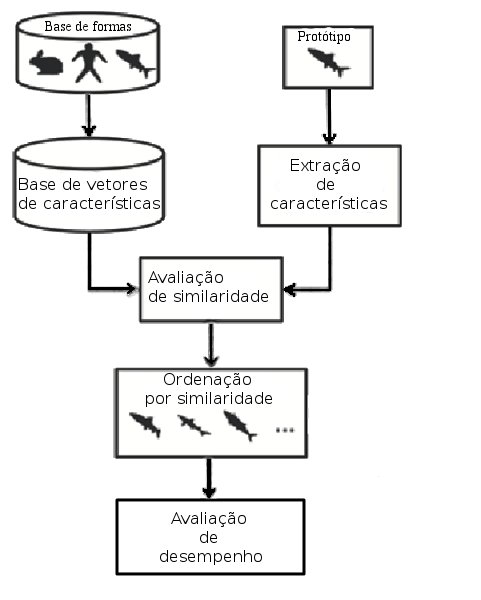
\includegraphics[width=0.55\textwidth]{Metodologia1.jpg}
\end{figure}

Na avaliação do desempenho dos experimentos duas medidas são utilizadas: o número total de acertos por posição recuperada e a medida Bull-eye.

A primeira medida consiste no número total de ocorrências de formas da mesma classe que a forma de consulta em cada posição recuperada.  Em diversos trabalhos de recuperação de formas pelo conteúdo o número total de acertos por posição recuperada é calculado para a base Kimia-99 \cite{Bernier:2003}. Tendo esta base 99 formas, igualmente distribuídas em 9 classes, são realizadas 99 recuperações das 11 formas mais similares à imagem de consulta. Como resultado espera-se obter um total de 99 formas recuperadas corretamente para cada posição recuperada.

A medida Bull-eye também é utilizada na literatura para a comparação de diferentes métodos de recuperação de formas. Essa medida é calculada para a base MPEG-7 CE-Shape-1 da seguinte maneira: tomando-se cada forma dessa base de imagens como elemento de consulta, contabiliza-se o número de recuperações pertencentes a mesma classe da forma de consulta dentre as 40 primeiras posições recuperadas. Como resultado calcula-se a percentagem da quantidade máxima de recuperações corretas possíveis de se alcançar, sendo esta última quantidade $28000 = 1400\text{ formas} \times 20\text{ recuperações corretas poro forma}$. 


\section{Avaliação de similaridade de formas}
 \label{Sec:method}
 
O método proposto para a avaliação de similaridade entre formas combina medidas de divergência com assinaturas do contorno das formas. A Figura \ref{fig:metodo_distancia} ilustra a metodologia aplicando-a a duas formas A e B. Uma vez extraído o contorno são calculadas quatro assinaturas daquelas abordadas na Seção \ref{sec:Assinatura} do Capítulo \ref{chap:contour}: curvatura \cite{149591,Costa:2009}, sequência de ângulos (AS) \cite{Fotopoulou:2013}, distância ao centróide (CD) \cite{Costa:2009} e invariante integral de área (AII) \cite{Manay:2006}. O próximo passo estima as distribuições de probabilidade dessas assinaturas através de histogramas. Um ponto considerado na determinação dos histogramas é o ajuste dos parâmetros utilizados na estimação das distribuições, que são o número de intervalos (bins) e a faixa de valores. Um número de intervalos grande torna a estimação sensível a ruído, enquanto um número pequeno desse parâmetro resulta em uma descrição com poder de discriminação pobre. Já a má escolha da faixa de valores resulta em perda de informação na descrição, o que também degrada o poder de discriminação.  Assim, a faixa de valores foi padronizada normalizando-se as assinaturas das formas, enquanto os números de intervalos (um parâmetro para cada assinatura) foram obtidos por otimização para maximizar o desempenho do descritor, conforme o método da Seção ??. 

Finalmente, as medidas de divergência $D(a,b)$ entre os histogramas correspondentes das formas A e B são calculados, resultando em quatro medidas de dissimilaridade, uma para cada par de assinaturas ($d_{1}$, $d_{2}$, $d_{3}$ e $d_{4}$), sendo a medida de dissimilaridade final $d(A,B) = d_{1}+d_{2}+d_{3}+d_{4}$. Cabe aqui mencionar que, por ser uma medida de dissimilaridade, quanto menor o valor de $d(A,B)$ maior a similaridade entre as formas $A$ e $B$. 

Realizou-se experimentos de recuperação de formas para avaliar o qualidade do método em questão para diferentes funções de divergência.

%A avaliação de similaridade entre formas a partir de medidas de divergência requer que as informações das assinaturas, abordadas na Seção \ref{sec:Assinatura} do Capítulo \ref{chap:contour}, sejam tratadas como variáveis aleatórias e que suas distribuições de probabilidade sejam estimadas. 

%A  Figura \ref{fig:metodo_distancia} ilustra como divergentes podem ser aplicados na avaliação da similaridade entre duas formas A e B. No método em questão, as distribuições de probabilidade de quatro assinaturas distintas dos contornos das formas são estimadas, através de histogramas, para em seguida se calcular as medidas de divergência. Uma medida de similaridade é então obtida  a partir da média ponderada das medidas de divergência.

\begin{figure}[h!]
  \caption{\label{fig:metodo_distancia} Método para avaliação da similaridade entre duas formas A e B utilizando distância estocástica e histogramas das assinaturas do contorno das formas.}
  \centering
  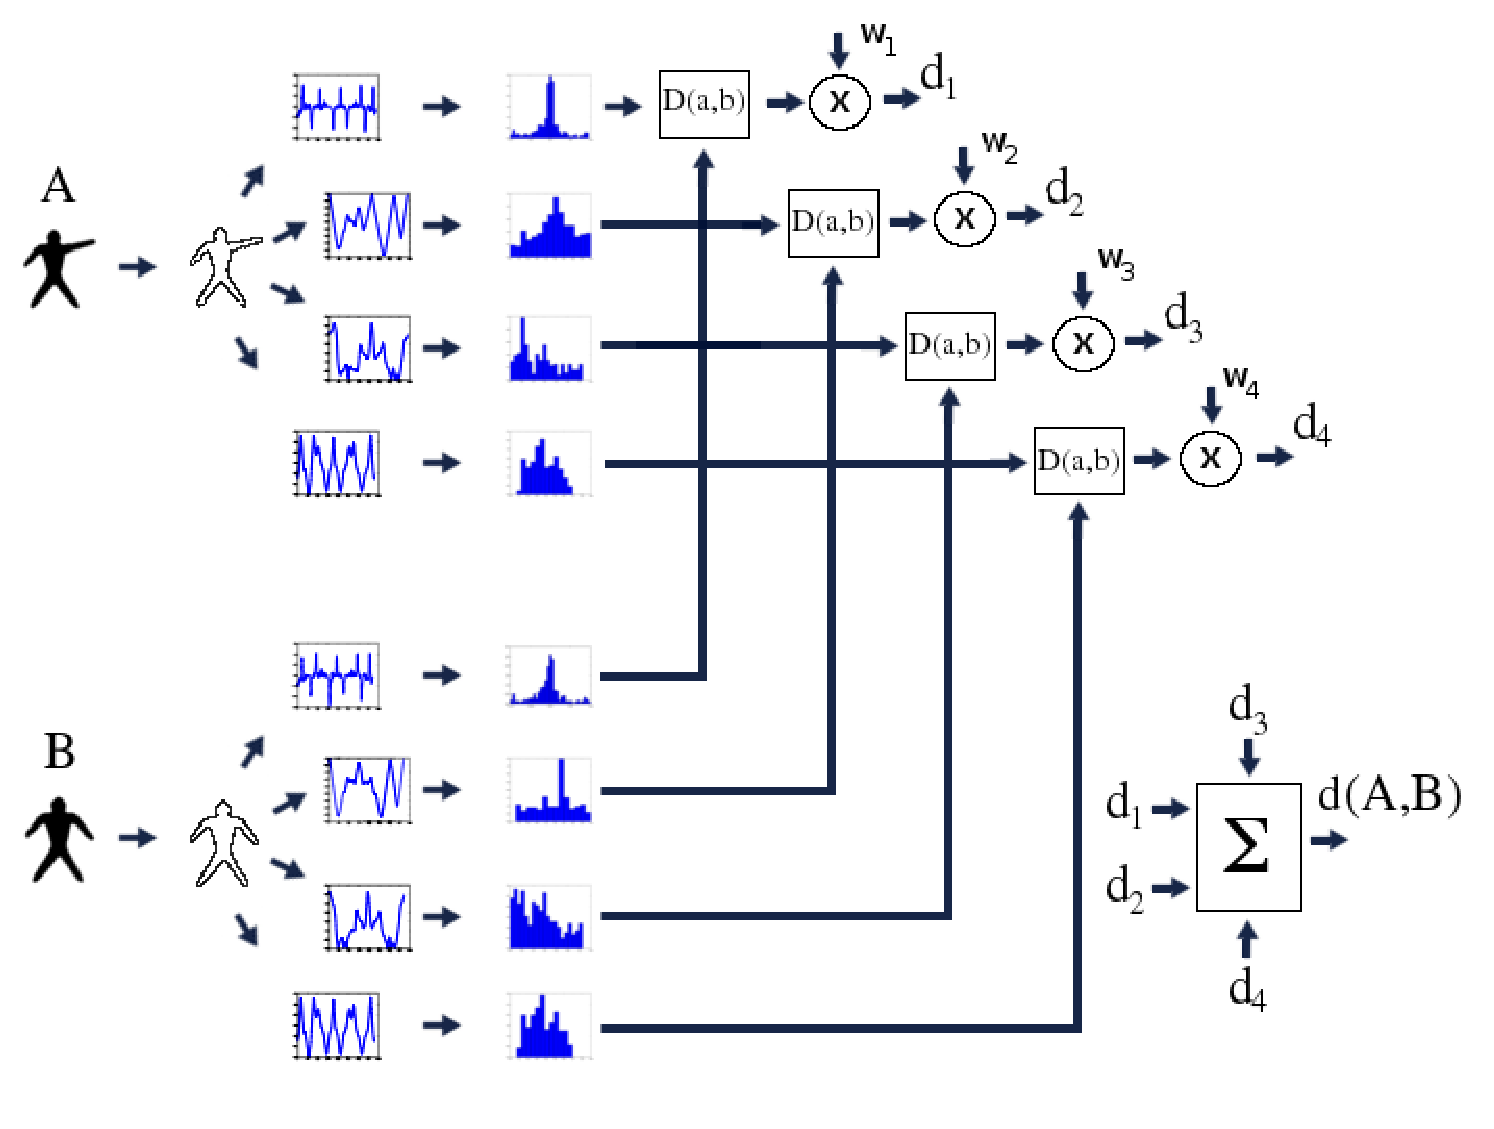
\includegraphics[width=0.85\textwidth]{figura_metodo.eps}
\end{figure}


\begin{comment}
\subsection{Visualizaçâo de dados}

A Figura \ref{fig:metodo_4} ilustra o método que empregamos na avaliação da capacidade discriminativa dos descritores de formas através das técnicas de visualização dos dados apresentadas.

\begin{figure}[h!]
  \caption{\label{fig:metodo_4} Método de avaliação de descritores multiescala do contorno de formas. (a) Base de imagens. (b) Extração de características. (c) Descritores de formas. (d) Análise de similaridade a partir da matriz-U. (e) Avaliação de agrupamentos a partir da medida silhouette.}
  \centering
  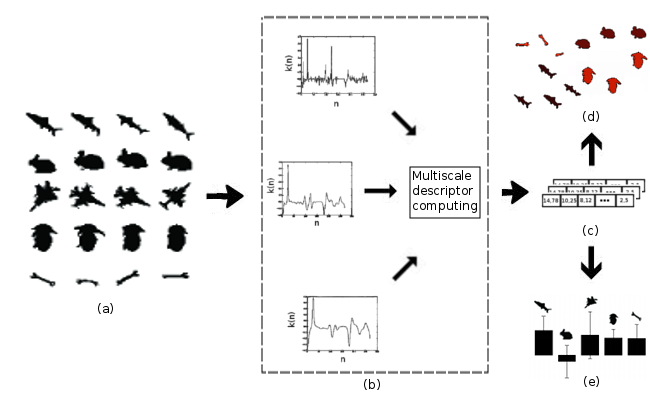
\includegraphics[width=0.75\textwidth]{metodo_v4.png}
\end{figure}

O primeiro passo consiste em realizar a extração de características num conjunto de formas binárias rotuladas (Figura \ref{fig:metodo_4}a e Figura \ref{fig:metodo_4}b) com o método de descrição sob análise. Como resultado temos um conjunto de descritores, ou vetores de características, das referidas formas (Figura \ref{fig:metodo_4}c). 

A avaliação de qualidade dos descritores se dá qualitativamente e quantitativamente. Na avaliação qualitativa (Figura \ref{fig:metodo_4}d) utilizamos a rede auto-organizável de Kohonen para obtenção da matriz de distâncias unificada, ou matriz-U. Essa última é empregada como ferramenta de visualização dos dados, o que possibilita identificar como o método de descrição sob avaliação agrupa as formas. 

Na avaliação quantitativa (Figura \ref{fig:metodo_4}e) utilizamos os rótulos e os vetores de características das formas para calculamos a medida de avaliação de agrupamentos \emph{Silhouette} \cite{Rousseeuw:1987}. Valores médios dessa medida, por classe de formas, indica a habilidade dos descritores em discriminar formas que pertençam a classes distintas e de agrupar formas que pertençam a uma mesma classe.
\end{comment}


\begin{comment}
\subsection{Self-organizing map and the U-matrix}

The self-organizing map, or SOM network \cite{Kohonen:2001}, is a neural network that performs nonlinear reduction of high-dimensional data by projecting it into a low-dimensional space. This method is an exploratory data analysis tool that has been used for image visualization \cite{Strong2011774}, cluster learning \cite{Kuroiwa200031} and texture classification \cite{595364}. 

A SOM network represents structural features of input data in a low-dimensional lattice. In fact, this tool displays data features in the lattice by using a neighborhood criterion in order to preserve structure of the input space.  According to \cite{Ultsch:1990}, the direct usage of this network output is not suitable for cluster analysis purposes.  The SOM network arranges clusters in different regions, although the distances among data points are uniformly distributed. To overcome this drawback, Ultsch and Siemon \cite{Ultsch:1990} developed a two-dimensional projection method, namely the unified distance matrix, i.e., the U-matrix. The U-matrix displays the local distance structure of a topology-preserving projection of a high-dimensional data set \cite{Ultsch:1990}.

\begin{figure}[!ht]
\centering
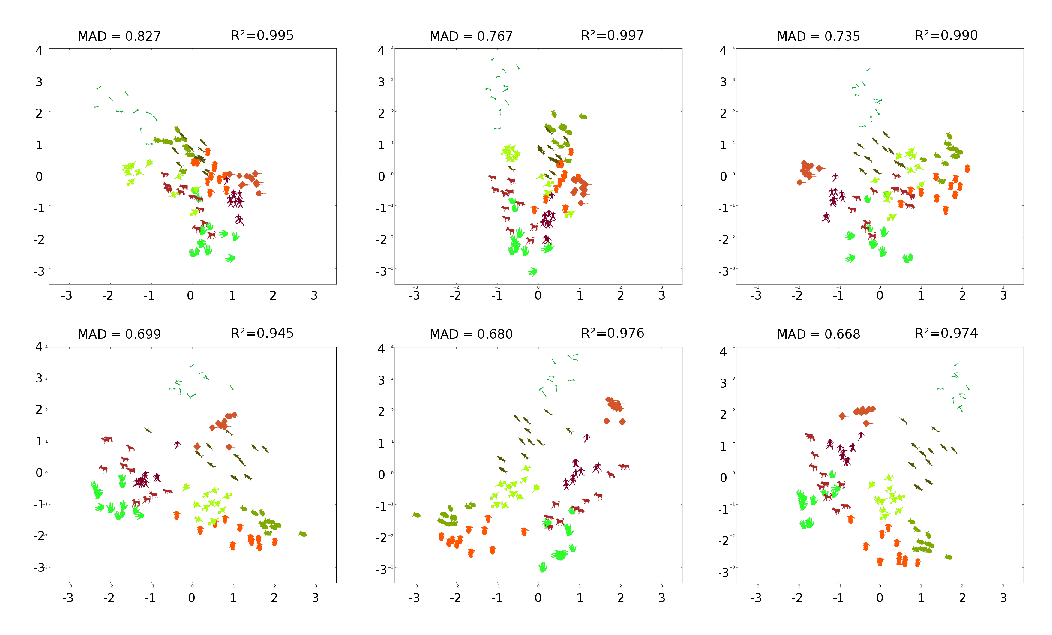
\includegraphics[width=0.75\textwidth]{fig4.eps}
\caption{\label{fig:projkimia99}U-matrices for shapes of MPEG7 CE-Shape-1 data set.}
\end{figure}

Figure \ref{fig:projkimia99} shows the U-Matrix for shapes of the MPEG-7 CE-Shape-1 data set \cite{855850}. The central image is the result of the whole data set described by the optimized NMBE.  The four images in the corners are details of the central image.
This visualization tool identifies how well NMBE describes subtle details from shapes of the same cluster and different clusters. In the detail images, we can observe the boundaries (in grey) which separate the well-defined shape clusters (e.g. clusters in the top-left corner image). Well-defined clusters are the ones with the lowest within-class and highest inter-class distances.

\section{Multidimensional Scaling (\emph{MDS})}
The multidimensional scaling \cite{cox:2000} searches for a low-dimensional data representation which preserves the distances of the original high-dimensional space. In general, this technique analyzes similarity or dissimilarity data. The MDS algorithm models similarity or dissimilarity data as distances in geometric spaces.

There exists two types of MDS algorithms: metric and non metric.  In the former, the input similarity matrix arises from a metric where the triangle inequality holds.  Thus, distances between two points are set to be as close as possible to the similarity or dissimilarity data. In the non-metric version, the algorithm  attempts to preserve the order of distances, and furthermore it seeks a monotonic relationship among the distances in the embedded space and the similarities/dissimilarities.

\begin{figure}[t]
\centering
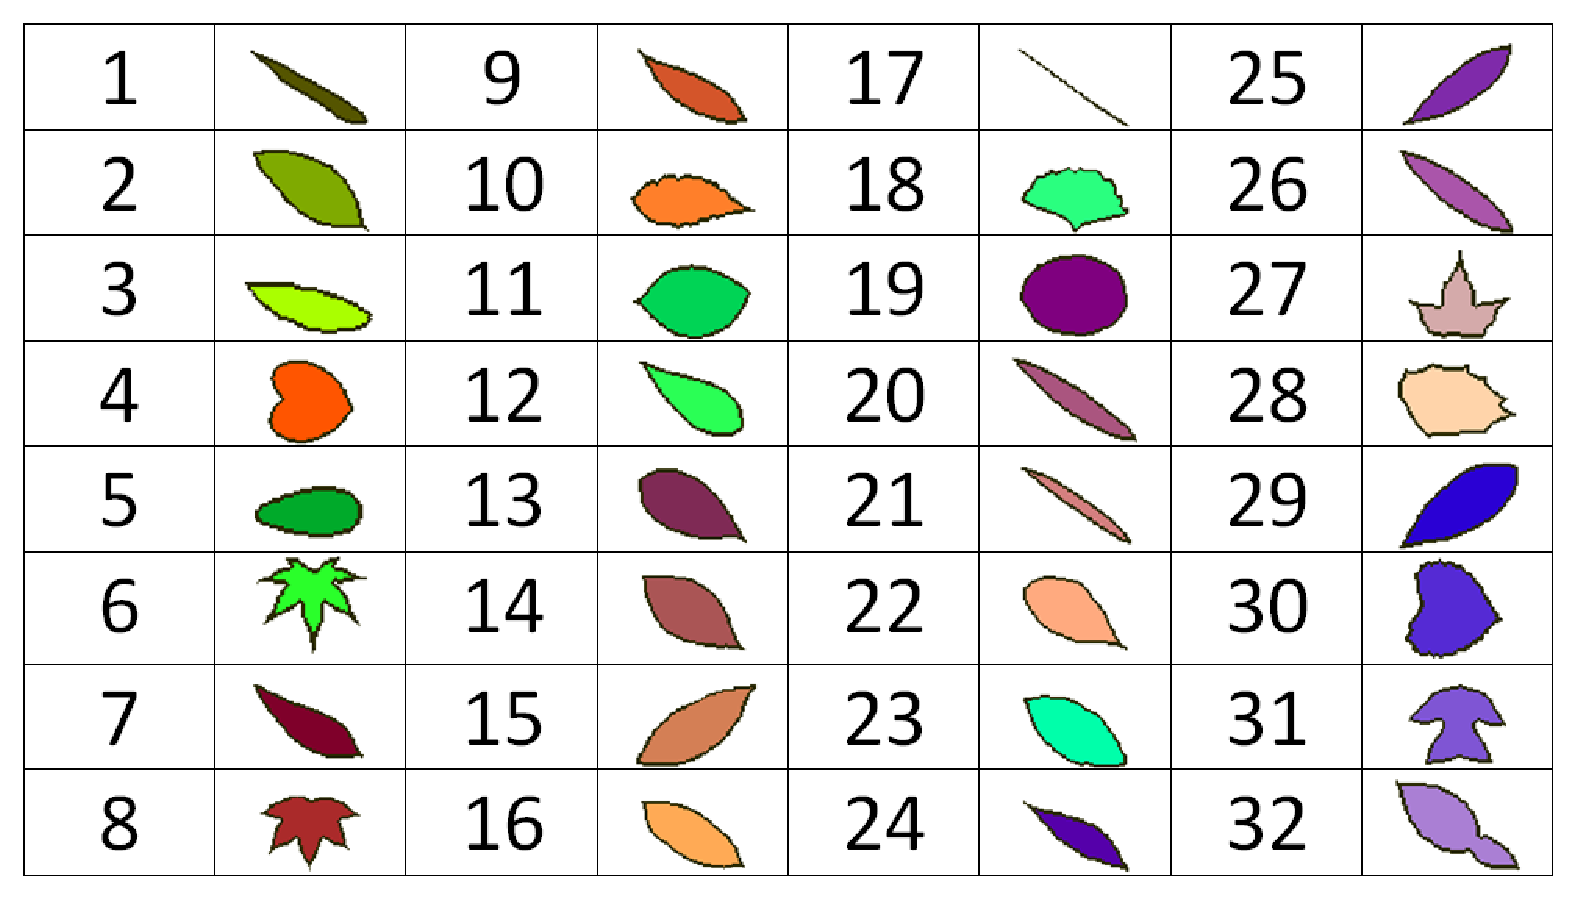
\includegraphics[width = 0.99\textwidth]{fig5.eps}
\caption{\label{fig:optimization_result} MDS projections of an experiment with $99$ shapes from Kimia data set \citeonline{Sebastian:2004}. The images display how clusters evolve during an optimization process (DE), as well as MAD and $R^2$ values.}
\end{figure}

The $R^2$ coefficient measures the fitness degree of the low-dimensional representation. This coefficient indicates, in percentage, the fitness of a model to the observed data. Thus, the closer the value of $R^2$ is to 1, the better the model fits the observed data. 

Let $d$ and $\hat{d}$ be the symmetrical distance matrices between feature vectors in the low and high-dimensional space. The $R^2$ coefficient is given by
\begin{equation}
R^2= 1-\frac{\sum_{i=1}^n \sum_{j = i}^{n}(\hat{d}_{i,j} - d_{i,j})^2}{\sum_{i=1}^n\sum_{j=i}^n (d_{i,j}-\bar{d})^2}
\text{,}\:\: R^2 \in [0,1]
\end{equation}

\noindent where $n$ is the number of samples, $d_{i,j}$ the distance between samples $i$ and $j$ in the high-dimensional space, $\hat{d}_{i,j}$ the distance between samples $i$ and $j$ in the low-dimensional space and $\bar{d}$ the mean distance in the high-dimensional space.

The MDS projections in Figure \ref{fig:optimization_result} illustrate how the shape clusters evolve as DE searches for the  optimized parameters of the shape descriptor (NMBE). The shape samples are from Kimia data set \cite{Sebastian:2004} which comprises $99$ shape images. Here, we have employed a manifold learning technique to produce the MDS projections of the optimized NMBE via DE. Figure \ref{fig:optimization_result} also shows that when the MAD values decreased, the inter-class distances increased and therefore the shape clusters became more evident.  At the minimum value of MAD, i.e., when the optimization process converged, the only clusters that were not well separated were the four-legged animals and the hand shapes. 

\end{comment}

We performed shape classification and retrieval experiments with the proposed optimization methodology by testing two descriptors on the Flavia data set \citeonline {4458016}, which comprises $1907$ leaf images with $32$ different species. Figure \ref{fig:bases} depicts leaf images taken from this challenging data set, which  presents a high between class similarity. This data set is widely used to validate automatic recognition systems of plant specimens. 

\begin{figure}[!htb]
\centering
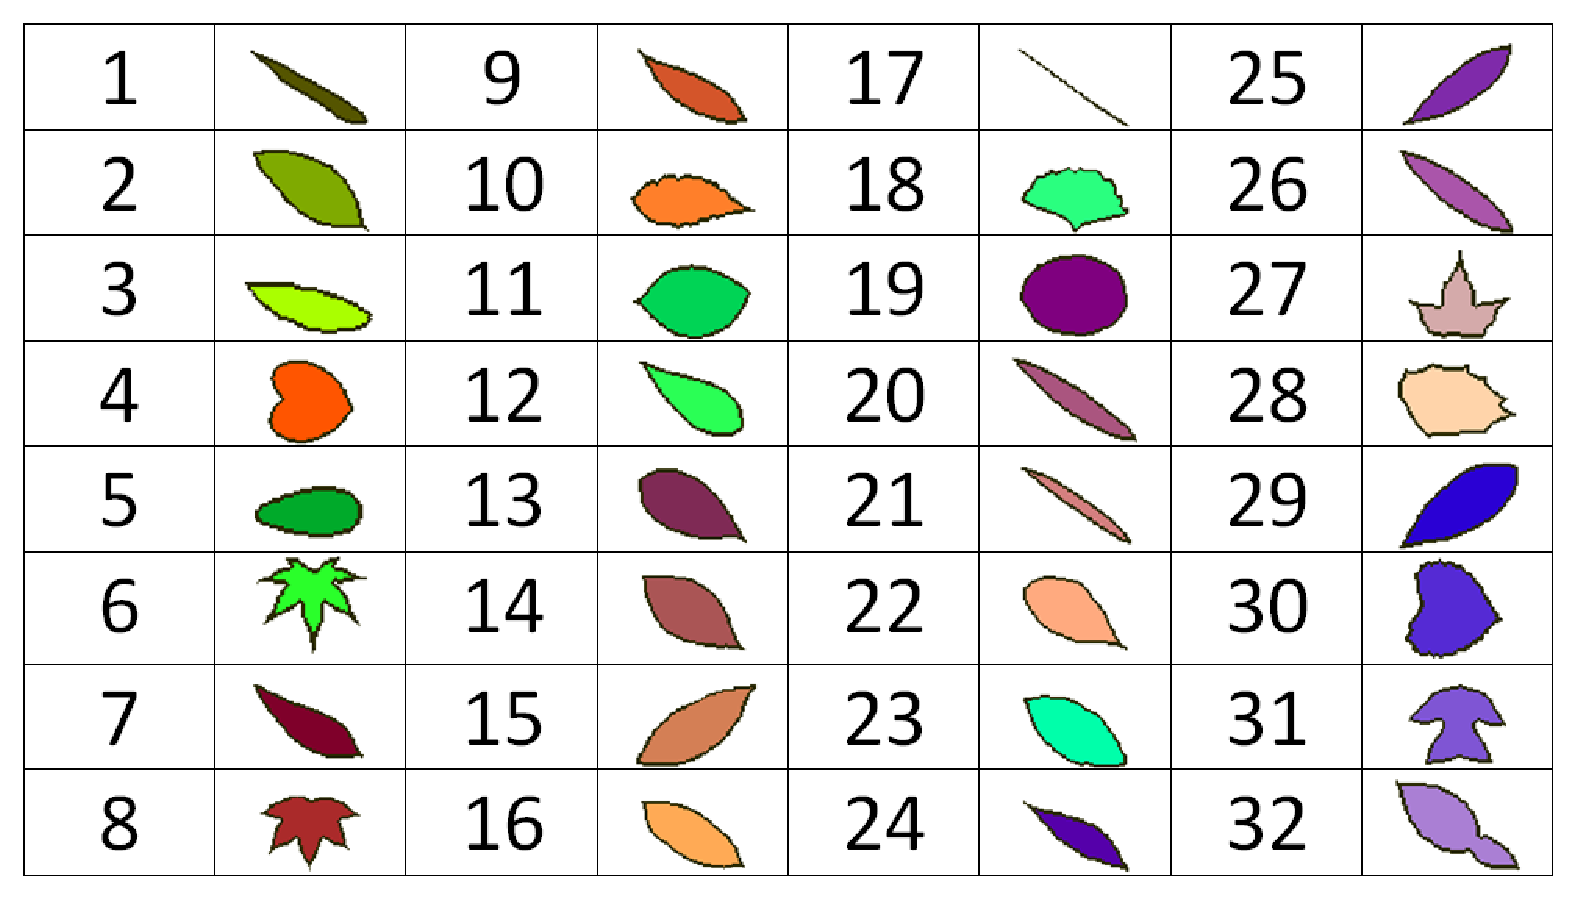
\includegraphics[width=0.3\textwidth]{fig5.eps}
\caption{\label{fig:bases}Samples of Flavia leaf data set.}
\end{figure}

\subsection{$MAD$ analysis and shape classification \label{sec:mad_class}}

Experiments were carried out to compare the optimization algorithms regarding convergence.  Figure \ref{fig:converge} illustrates the convergence of each optimization algorithm for $30$ runs on a subset of leaf shapes. 
The optimization results indicate that PSO required a smaller number of iterations to converge to an optimal solution, whereas SA and DE required a larger number of iterations. Since convergence aspects are closely related
to the number of iterations required to achieve an optimal solution, few iterations imply poor exploration of the search space, thus leading to premature convergence \citeonline{Andries:2007}. In such case, the optimization method tends to get stuck in local minimums finding sub-optimal solutions. On the other hand, slower convergence enables the optimization method to explore more the search space, thus increasing the chance to converge to global minima, i.e. optimal solutions \citeonline{Andries:2007}. 
In this context, PSO hit more frequently in sub-optimal solutions, reaching a higher mean MAD value of 
$0.805 \pm 0.006$. On the other hand, SA and DE achieved lower mean 
MAD values of $0.795 \pm 0.006$ and $0.798 \pm 0.004$, respectively. 

In this context, the experimental results demonstrated that SA and DE were more efficient than PSO to find an optimal solution. However, the computational cost evaluation indicated that SA was less expensive than DE since the former evaluated the objective function less times than the latter.  Section \ref{sec:comp_cost} addresses more details about the computational cost of the optimization algorithms.

\begin{figure}[!htb]
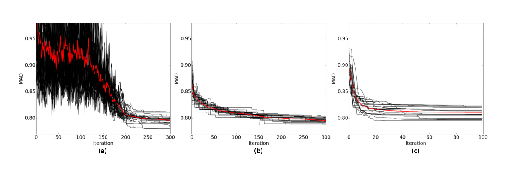
\includegraphics[width = \textwidth]{fig6.eps}
\caption{\label{fig:converge}Convergence of the optimization methods: (a) SA, (b) DE, (c) PSO. The red lines in each graphic refer to the mean MAD value of 30 runs (black lines) for the results of each optimization strategy within a subset of leaf shapes.}
\end{figure}

\begin{table}[hb!]
\begin{minipage}{\textwidth}
\renewcommand\footnoterule{}
\caption{Different MAD values and the classification results for different scale selection strategies for Flavia leaf data set.}
\label{tab:leaves_supervised_results}
\resizebox{\textwidth}{!}{ 
\begin{tabular}{cccccccccc}
\toprule[1.5pt]
 & \multicolumn{8}{c}{Classifier} \\ \cmidrule(lr){2-9} 
 & \multicolumn{2}{c}{NB}  & \multicolumn{2}{c}{Knn (n = 5)}  & \multicolumn{2}{c}{LDA}  & \multicolumn{2}{c}{QDA} \\
\cmidrule(lr){2-3}  \cmidrule(lr){4-5} \cmidrule(lr){6-7}  \cmidrule(lr){8-9}
MAD & Precision & Recall & Precision & Recall & Precision & Recall & Precision & Recall \\ \midrule
$0.762$\footnote{Using SA}        & ${0.91 \pm 0.02}$   & ${0.89 \pm 0.02}$         & ${0.93 \pm 0.02}$          & ${0.92 \pm 0.02}$         & ${0.87  \pm 0.02}$          & ${0.85\pm 0.02}$         & ${0.95  \pm 0.01}$          & ${0.94  \pm 0.01}$         \\
$0.783$\footnote{Using DE}        & $0.88 \pm 0.02$          & $0.87\pm0.02$         & $0.90\pm0.02$          & $0.88\pm0.02$         & $0.85\pm0.02$          & $0.83\pm0.03$         & $0.91\pm0.02$          & $0.90\pm0.02$         \\
$0.829$\footnote{Using PSO}        & $0.86\pm0.03$          & $0.85\pm0.03$         & $0.89\pm0.03$          & $0.88\pm0.03$         & $0.84\pm0.03$         & $0.82\pm0.03$         & $0.91\pm0.02$          & $0.89\pm0.02$         \\
{$0.867$\footnote{Using scales proposed by \citeonline{Cesar:1996}}}          & $0.85\pm0.02$          & $0.84\pm0.02$         & $0.89\pm0.02$          & $0.88\pm0.02$         & $0.82\pm0.03$          & $0.81\pm0.03$         & $0.89\pm0.02$          & $0.88\pm0.02$         \\
{$0.969$\footnote{\label{note1}Random selection}}          & $0.81\pm0.03$          & $0.79\pm0.03$         & $0.87\pm0.02$          & $0.85\pm0.02$         & $0.77\pm0.03$          & $0.77\pm0.03$         & $0.87\pm0.03$          & $0.85\pm0.03$         \\
{$1.04$\footref{note1}}          & $0.69\pm0.03$          & $0.68\pm0.03$         & $0.83\pm0.03$          & $0.82\pm0.03$         & $0.74\pm0.03$          & $0.73\pm0.03$         & $0.81\pm0.03$          & $0.79\pm0.03$         \\
\bottomrule[1.5pt]
\end{tabular}}
\end{minipage}
\end{table}

Our next analysis concentrates on the assumption that the optimized scales and the minimum values of MAD, which are intertwined, lead to an increase of the correct classification rate.
Table \ref{tab:leaves_supervised_results} presents different MAD values and their corresponding classification results. The optimized scales which attained the best classification results correspond to the minimum values of MAD. The NMBE descriptor whose scales were adjusted according to \citeonline{Costa:1997} ($\operatorname{NMBE_{orig}}$) led the classifiers to reach an intermediate performance. The optimized NMBE ($\operatorname{NMBE_{opt}}$) improved the performance of all classifiers since they accomplished the highest Precision and Recall rates when the objective function reached the minimum values. Thus, we can state that there is an intrinsic relation between the high correct classification rates and minimum MAD values.
Although the optimization algorithms achieved different MAD values and therefore different sets of optimized scales, the classification experiments showed that these scales captured leaf shape details and variations. Such results confirmed that we can take advantage of the optimization algorithms to strengthen leaf shape characterization and analysis. 
In spite of NMBE has been originally designed for neural cell description, this paper focus on leaf shape characterization. Moreover, the proposed objective function tailored NMBE in terms of scales to the problem and leaf shape data set under analysis, satisfactorily. 
  
The classifiers that used the non-optimized NMBE with randomly selected scales did not perform well since they have reached the lowest values for Precision and Recall and the highest values for the objective function (MAD). 
Thus, we concluded that randomly selected scales were less sensitive to leaf shape variations and tended to provide more misclassifications. 

\subsection{Visual exploratory cluster analysis}
The visual exploratory cluster analysis indicates that the optimized descriptor improves the cluster arrangement of leaf shapes, which reinforces that MAD is an objective function suitable to guide parameter optimization. 
Figure \ref{fig:MatrizU_leaves_256}  depicts the U-matrices that support the visualization of leaf shapes. The leaf colors are in accordance with the class labels exhibited in Figure \ref {fig:bases}. These U-matrices comprise $1907$ leaf shapes, and furthermore each leaf is represented by its descriptor. 

Figure \ref{fig:MatrizU_leaves_256}a shows leaf shapes which are described by the optimized NMBE, while Figure \ref{fig:MatrizU_leaves_256}b displays, in terms of U-matrix elements, leaf shapes described by the non-optimized NMBE descriptor.  The graphical representations of the \emph{silhouette}  measure in Figures \ref{fig:MatrizU_leaves_256}a and \ref{fig:MatrizU_leaves_256}b demonstrated that the leaf classes, which were properly characterized and grouped, were those with positive mean \emph{silhouette} values. Nevertheless, leaf shapes whose descriptors were not able to characterize and group them properly were those with negative  \emph{silhouette} values. Figure \ref{fig:MatrizU_leaves_256}a shows the remarkable  reduction of negative mean \emph{silhouette} values when applying $\operatorname{NMBE_{opt}}$ to shapes from Flavia leaf data set. 

\begin{figure}[t]
\centering
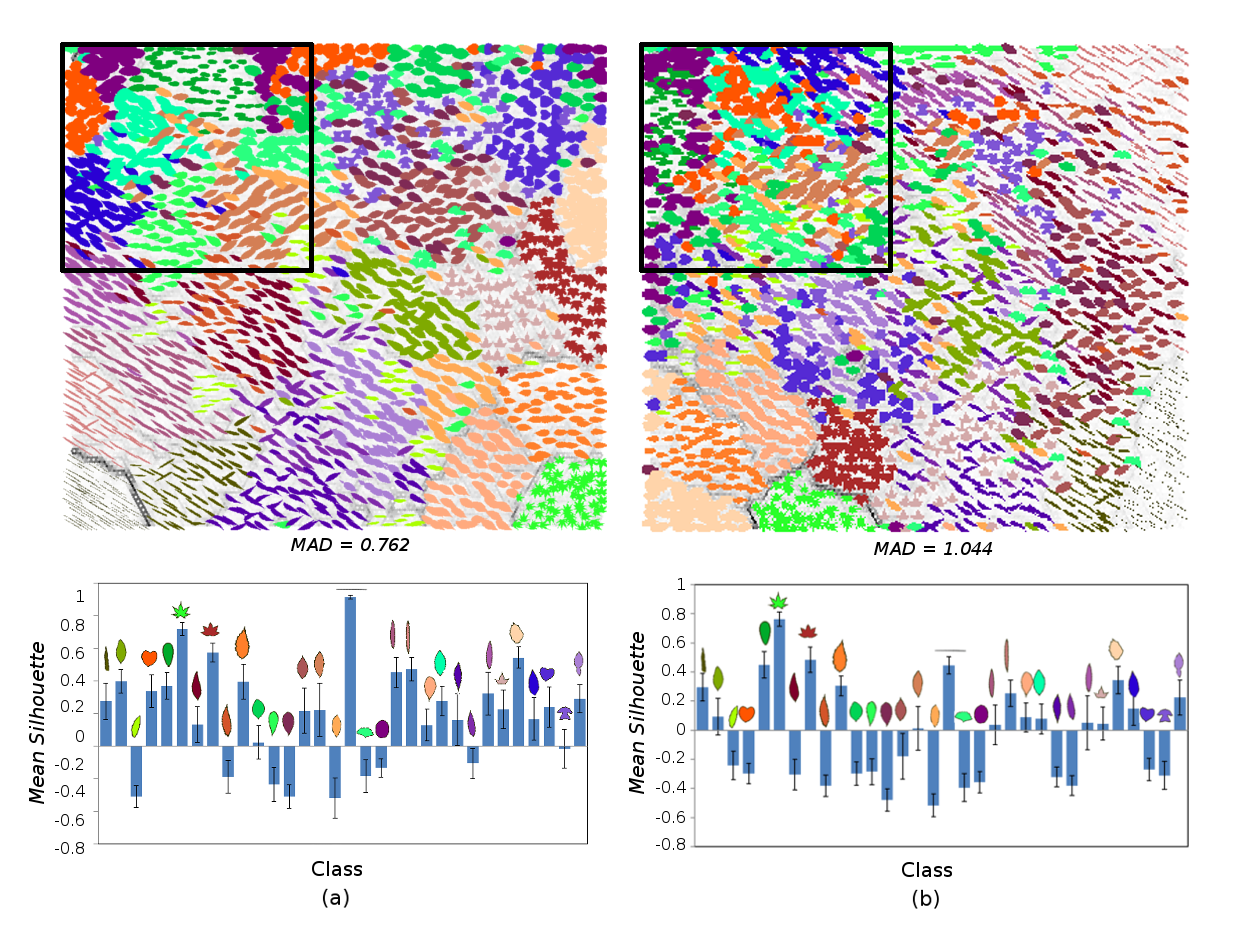
\includegraphics[width=0.75\textwidth]{fig7.eps}
 \caption{\label{fig:MatrizU_leaves_256}U-matrices and mean \emph{silhouette} measure for Flavia leaf data set using the (a) optimized and (b) non-optimized NMBE.}
\end{figure}

The black square in Figure \ref{fig:MatrizU_leaves_256}a highlights  the performance of the optimized descriptor. It also shows how well the optimized descriptor mapped leaf shapes into groups according to their respective classes.  Moreover, the optimized descriptor has remarkably improved  the mean \emph{silhouette} per class for almost all leaf classes. In contrast, the region inside the black square in Figure \ref{fig:MatrizU_leaves_256}b indicates that the non-optimized descriptor was unable to satisfactorily map leaf shapes in their corresponding classes.
These results  indicated that the optimized descriptor has improved the cluster arrangement of leaves due to the intrinsic shape variations within the set of optimized scales that can not be properly embodied in the studied traditional parameter selection methods.

Figures \ref{fig:MatrizU_leaves_II}a, \ref{fig:MatrizU_leaves_II}b and \ref{fig:MatrizU_leaves_II}c display the U-matrices and the corresponding MAD values for experiments on Flavia leaf data set with SA, DE and PSO, respectively. An interesting aspect to examine in these results regards the convergence of the optimization algorithms to different solutions (MAD). These solutions resulted in different cluster arrangements and therefore different relations among the neighborhood structure of clusters. For instance, the overall dispersion  of the elements in Figure \ref{fig:MatrizU_leaves_II}a and Figure \ref{fig:MatrizU_leaves_II}b tend to be very similar since  the corresponding MAD values are close to each other. At the same time, the result that corresponds to the highest MAD value ($0.829$) exhibits a relatively high dispersion within clusters, particularly at the center of the U-matrix (Figure \ref{fig:MatrizU_leaves_II}c), which reinforces the hypothesis that  PSO converged to a local minimum. These findings point to the important conclusion that the lower the MAD value, the better the cluster arrangement and hence the cluster quality. Therefore, we state that the cluster quality and MAD value are negatively correlated. Our analysis also considers that there are other solutions than the minimum, in the search space, which may be suitable to the problem under study. 

\begin{figure}[h!]
\centering
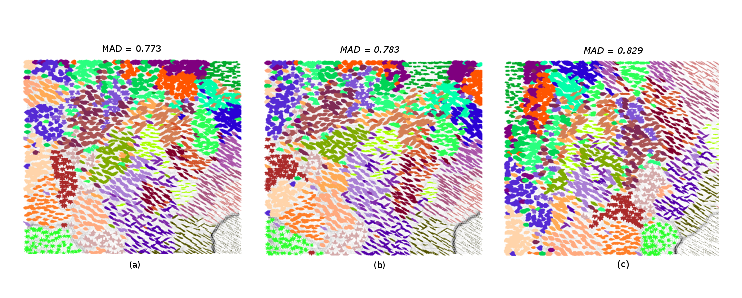
\includegraphics[width=\textwidth,trim = 0mm 0mm 0mm 4.5mm,clip]{fig8.eps}
 \caption{\label{fig:MatrizU_leaves_II}U-matrices and MAD values for Flavia leaf data set achieved by using  the optimized NMBE with (a) SA, (b) DE, (c) PSO.}
\end{figure}

Figure \ref{MDS:Leaves} illustrates the MDS projections for three different MAD values. Figure \ref{MDS:Leaves}a corresponds to the cluster arrangement after the convergence of the SA algorithm, i.e. after reaching the minimum MAD value. These projections confirmed that the minimization of the objective function provided leaf cluster arrangements with lower average within-class distances and higher inter-class distances, and thus  more compact and separated clusters. The visual analysis of the three detail images in Figure \ref{MDS:Leaves}a discloses that the MDS projection of the optimized NMBE descriptor increased inter-class distances, whereas it reduced the within-class distances when compared to Figure \ref{MDS:Leaves}b and \ref{MDS:Leaves}c. Moreover, the $R^2$ coefficient values close to 1 imply that the low-dimensional representation preserved the mean distance in the original high-dimensional data space.

\begin{figure}[h!]
\centering
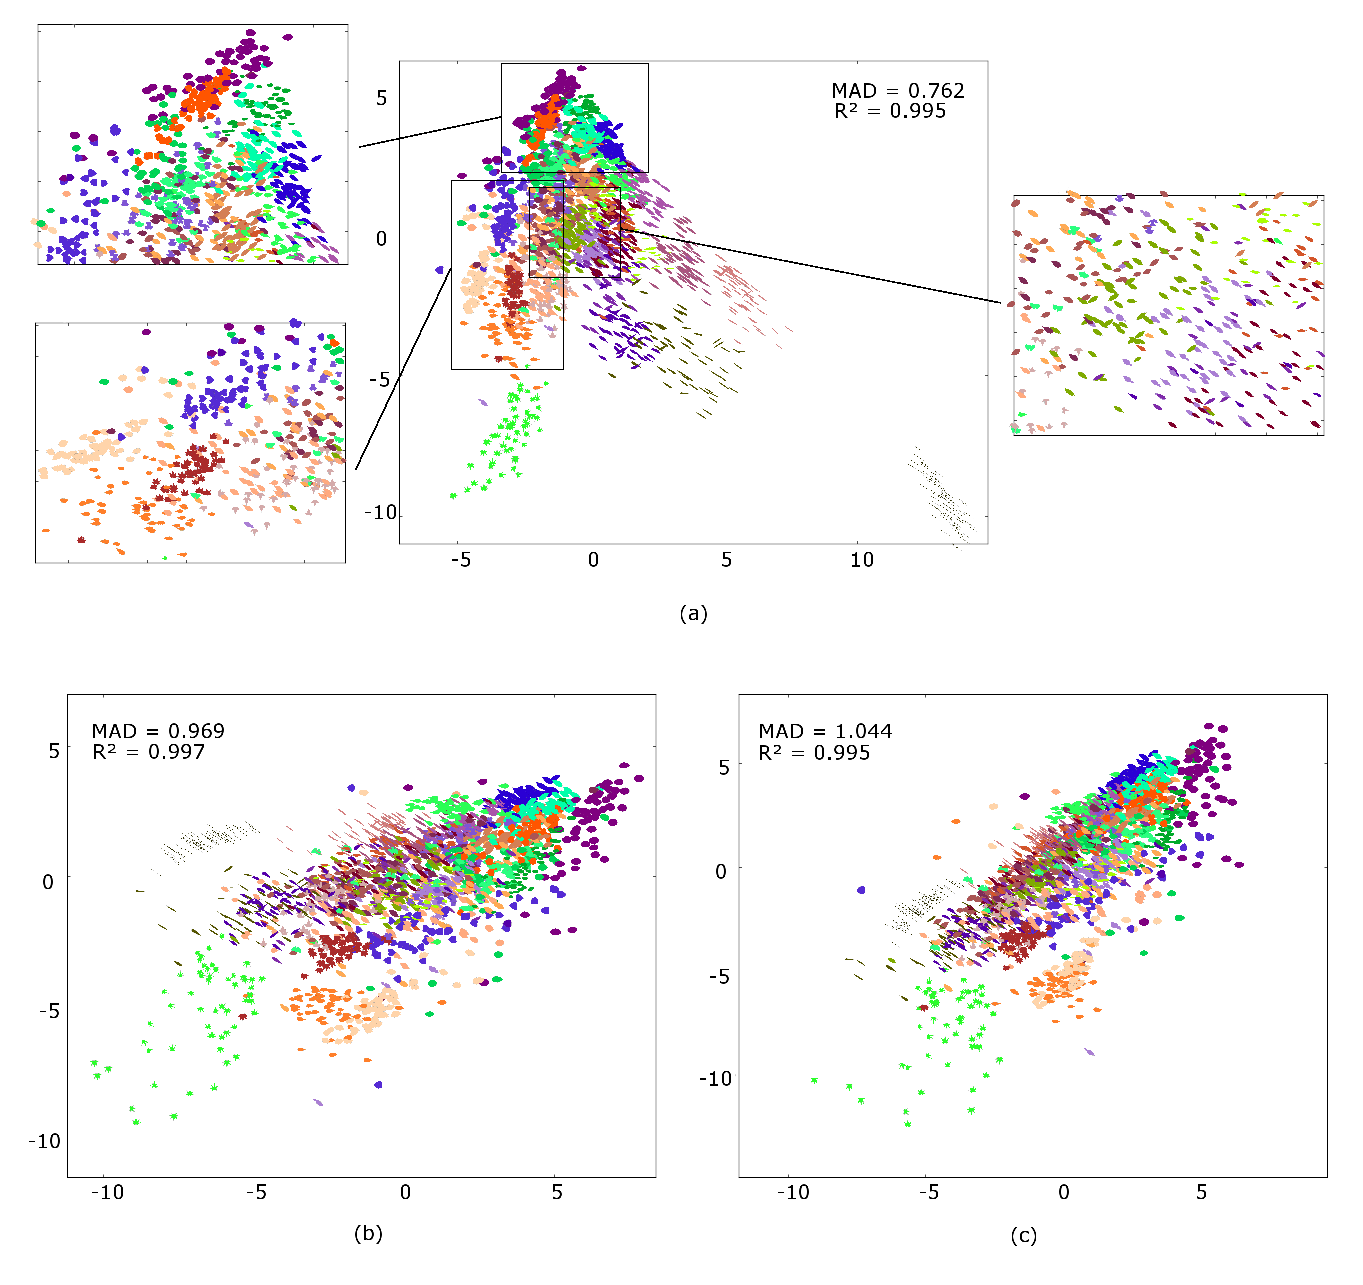
\includegraphics[width=0.75\textwidth]{fig9.eps}
 \caption{\label{MDS:Leaves} MDS projections of the NMBE descriptors for leaf shapes of Flavia data set. (a) The SA-optimized NMBE descriptor with $MAD = 0.762$ (b) non-optimized NMBE with $MAD =0.969$ and (c) non-optimized NMBE with $MAD = 1.044$ }
\end{figure}

\subsection{Shape retrieval experiment}
For the sake of comparison, we have optimized the parameters of another shape descriptor namely inner distance shape context (IDSC) \citeonline{Ling:2007:SCU:1191552.1191806}.
This descriptor is mainly applied to shape retrieval, which involves unsupervised shape classification tasks.  Moreover, IDSC employs dynamic programming (DP), such as Dynamic Time Warping (DTW) \citeonline{PalazonGonzalez2012978}, to improve shape matching accuracy. In this paper, we have replaced the $L_2$ norm by DTW to compute the \emph{silhouette} measure and the cost function defined in equation \ref{eq:mad}.  
Figure \ref{figfig1Optmization-IDSC} exhibits the comparison of shape retrieval experiments which were performed on the public Flavia leaf data set and with both non-optimized NMBE and IDSC and their optimized counterparts ($\operatorname{NMBE_{opt}}$, $\operatorname{IDSC_{opt}}$).
The performance evaluation methodology has adapted the Bulls-eye measure, where the result is the overall number of shapes correctly  retrieved, in each rank position, for each shape in data set taken as a query.  Let $N_c$ be the number of shapes which belong to the class $c$. Here, the number of retrieved shapes ($N_r$) was adjusted to $N_r = 2\displaystyle \min_{c = 1,2,\dots 32}{N_c}$. Figure \ref{figfig1Optmization-IDSC} also demonstrates that the optimization methodology was decisive for both descriptors to achieve better retrieval rates. 
Figure \ref{fig1Ooptimization_graph}  shows that after tuning IDSC parameters for the Flavia leaf data set with the optimization methodology the retrieval rate has remarkably increased. Therefore, $\operatorname{IDSC_{opt}}$  outperformed the optimized NMBE ($\operatorname{NMBE_{opt}}$) and non-optimized NMBE. In this sense, the optimized parameters of $\operatorname{IDSC_{opt}}$ may have incorporated subtle details of leaf shapes. On the other hand, we have observed that the non-optimized IDSC underperformed the non-optimized NMBE. 
In order to provide a non-optimized counterpart of IDSC, we have followed the parameter setting introduced in \citeonline{wang2015march}.
Figure \ref{subfig:upper-right} and \ref{subfig:lower-right} exemplify samples of  plant leaves which were retrieved according to the rank of the similarity to the two queries. These results have demonstrated that the non-optimized descriptors in Figure \ref{subfig:upper-right} and \ref{subfig:lower-right} were unable to retrieve all samples for the two queries, whereas the  optimized descriptors retrieved all of them, correctly.
\begin{comment}
\begin{figure}[t!]
\begin{subfigure}{0.55\textwidth}
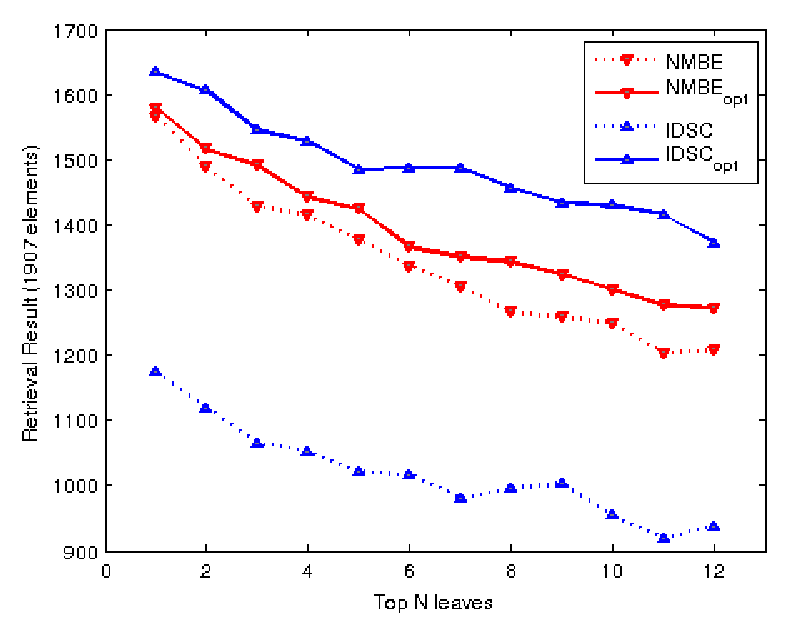
\includegraphics[width=\textwidth]{fig10a.eps}
\caption{Retrieval rates. \label{fig1Ooptimization_graph}}
\end{subfigure}
\hspace*{\fill}
\begin{minipage}{0.45\textwidth}
\begin{subfigure}{\textwidth}
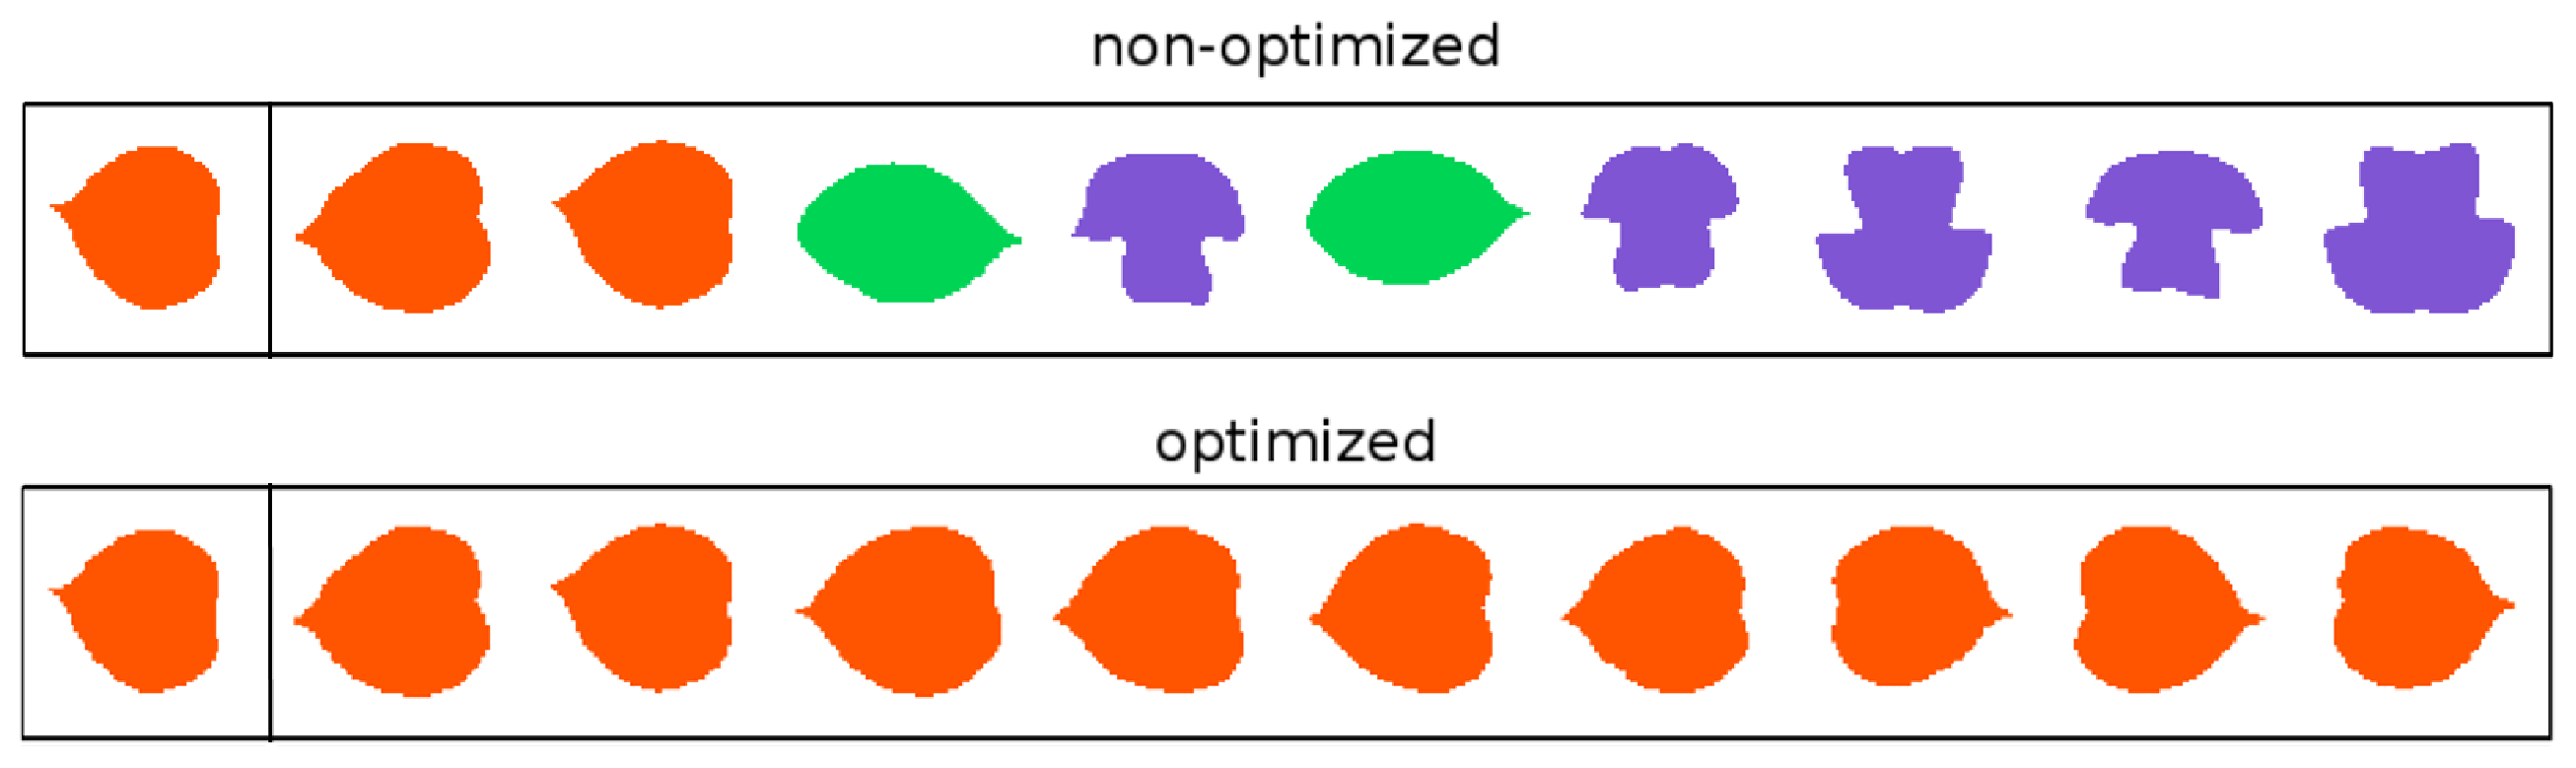
\includegraphics[width=\textwidth]{fig10b.eps}
\caption{Retrieval results with NMBE.} \label{subfig:upper-right}

\end{subfigure}

\vspace*{0.60cm}
\begin{subfigure}{\textwidth}
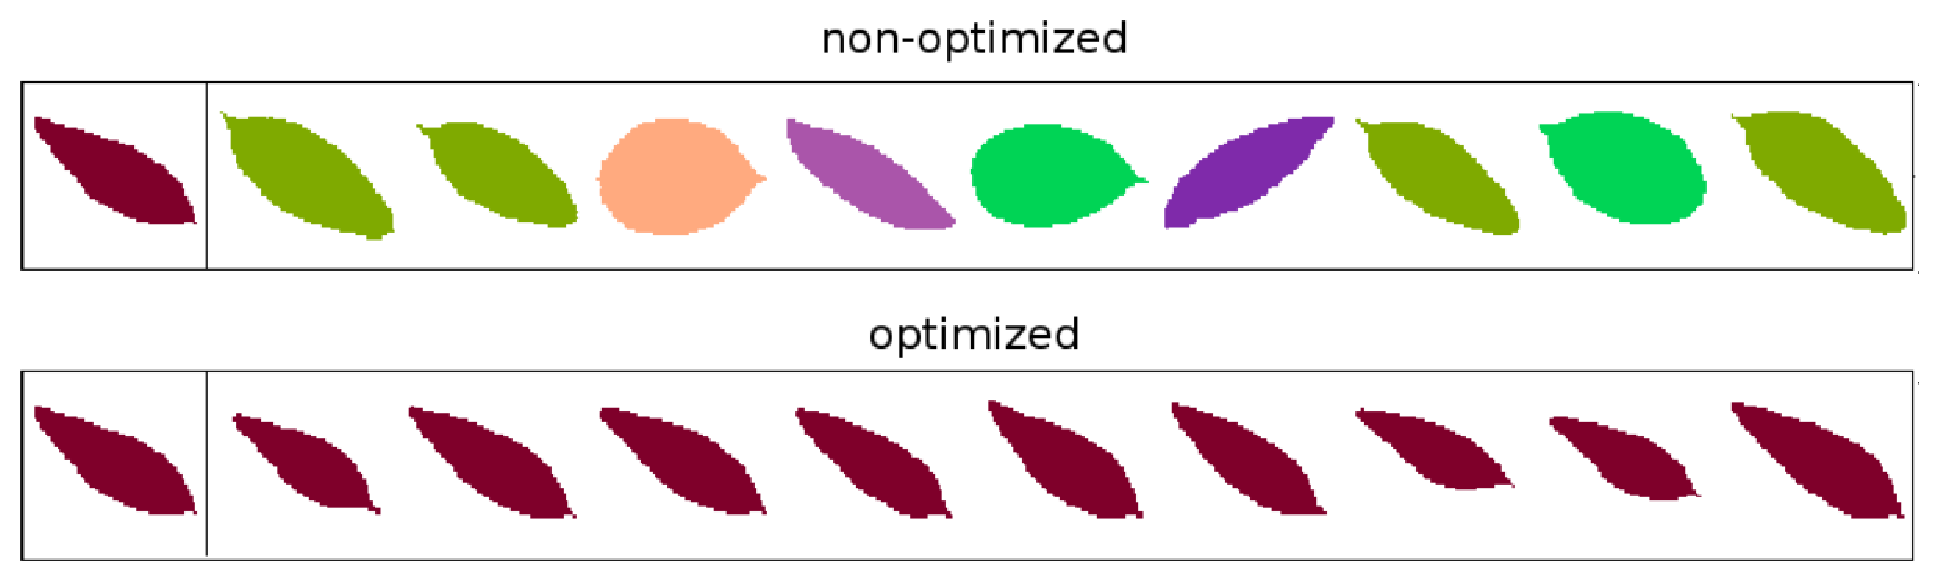
\includegraphics[width=\textwidth]{fig10c.eps}
\caption{Retrieval results with IDSC.\label{subfig:lower-right}}
\end{subfigure}
\end{minipage}

\caption{\label{figfig1Optmization-IDSC} Experiments conducted on Flavia leaf data set (a) retrieval rate by using both NMBE and IDSC and their optimized counterparts, (b) and (c) two leaf shape retrieval examples by using the non-optimized and optimized NMBE and IDSC descriptors, respectively.} 
\end{figure}
\end{comment}

 Table \ref{table_bull_eyes_leaves} presents the performance evaluation of NMBE, whose scales were computed using the scheme introduced by \citeonline{Cesar:1996}, IDSC and their optimized counterparts.  The retrieval rates show that both optimized descriptors outperformed their non-optimized counterparts on Flavia data set. The remarkable improvement on the Bulls-eye rates reinforces our assumption that the optimization methodology is suitable for leaf shape retrieval and analysis.

\begin{table}[h!]
\centering
\caption{Bulls-eye scores for Flavia data set.}
\label{table_bull_eyes_leaves}
  \begin{tabular}{cccccccc}
  \toprule[1.5pt]
 $\operatorname{NMBE}$ & $\operatorname{NMBE_{opt}}$ & IDSC    & $\operatorname{IDSC_{opt}}$\\ \midrule
     63.86 \%  & 71.16 \%  & 53.38\%    & 77.50\%       \\
  \bottomrule[1.5pt]
  \end{tabular}
\end{table}

Thus, we can infer that the optimized descriptors are more likely to succeed in shape retrieval experiments because the optimized sets of parameters probably embody intrinsic and subtle information about leaf shapes. We can also assume that these optimized descriptors may reliably characterize and also discriminate shape differences within and among leaf classes. 

\subsection{Computational cost \label{sec:comp_cost}}

Table \ref{tbl:complexity} shows the computational complexity results of the three optimization algorithms. SA and PSO present similar complexity results which rely on the number of iterations to converge ($N_{iter}$), population size ($N_{pop}$) and $P$ parameter. On the other hand,  DE  demands a higher complexity which relies on the dimension of the optimization problem ($D$), population size ($N_{pop}$) and number of iterations to converge ($N_{iter}$).

\begin{table}[h!]
\centering
\caption{Computational complexity of the optimization methods.}
\label{tbl:complexity}
  \begin{tabular}{ll}
  \toprule[1.5pt]
 Method & Complexity\\
 \midrule
   SA  & $O(P.N_{iter}.\log{N_{iter}})$    \\
   DE  & $O(N_{pop}.N_{iter}.D)$   \\
   PSO&  $O(N_{pop}.N_{iter}.\log{N_{iter}})$\\
  \bottomrule[1.5pt]
  \end{tabular}
\end{table}

For the sake of comparison, we assumed that the computational cost is the number of times that the objective function is demanded throughout the optimization process. Its calculation takes into account the parameter setting of each method, presented in Section \ref{subsec:opmet}, and the corresponding computational complexity.  The computational cost to address the optimization of the multiscale descriptor for SA, DE and PSO yielded $7,4314$, $19,500$ and $1,107$, respectively. 

It is worth noting that there is a trade-off between the computational cost and the quality of the optimal solution found. Although the reduction of the number of shape samples, image resolution and the $N_{pop}$ variable can lessen the computational cost, it may degrade the optimization result. Moreover, parallelism may contribute to reduce the computational cost without degrading the optimization result.  However, it adds an extra computational complexity to the optimization algorithms.
